
\documentclass[11pt a4paper]{article}
\usepackage[margin=2cm]{geometry}
\usepackage{amsmath, amssymb}
\usepackage{graphicx}
\usepackage{float}
\usepackage{aligned-overset}
\usepackage{subcaption}
\usepackage{tabularx} % fuer gleichungen nebeneinander
\usepackage{wrapfig} % damit figures neben text sien koennen

% partielle ableitungen
\newcommand{\delr}{\partial_r}
\newcommand{\deltheta}{\partial_\theta}
\newcommand{\delphi}{\partial_\varphi}

% elektrische feldkonstante
\newcommand{\epsz}{\epsilon_0}
% 1 / 4pi eps
\newcommand{\kco}{\frac{1}{4\pi\epsilon_0}}

% rotation
\newcommand{\rot}{\text{rot}}
\newcommand{\arsinh}{\text{arsinh}}

% fancy header
\usepackage{fancyhdr}
\fancyhf{}
% vspaces in den headern fuer Distanzen notwendig
% linke Seite: Namen der Abgabegruppe
\lhead{\textbf{Matthias Maile\\Roman Surma}\vspace{1.5cm}}
% rechte Seite: Modul, Gruppe, Semester
\rhead{\textbf{Physik II - Gruppe 2\\Sommersemester 2020}\vspace{1.5cm}}
% Center: nr. des blattes
\chead{\vspace{2.5cm}\huge{\textbf{20. Übungsblatt}}}
% benoetigt damit der eigentliche Text nicht in der Überschrift steckt
\setlength{\headheight}{4cm}

% zum zeichnen tikz
\usepackage{tikz}

% fuer fabigen text
\usepackage{xcolor}

% irgendwas mit figures
\usepackage{subcaption}

\begin{document}
\thispagestyle{fancy}
\section*{Aufgabe 1}
Im Bereich des Magnetfeldes wirkt eine Lorentzkraft, welche eine Spannung induziert. Diese Spannung ermitteln wir, 
indem wir ein Elektrisches Feld gegen die Lorentzkraft setzen, welche sich ausgleichen. Das Wegintegral des
$E$-Feldes ist dann die Induktionsspannung $U_\text{ind}$.
\begin{align*}
	F_\text{Lo}
	&= \vert \vec v \times \vec B \vert \quad \\ 
	% in skalaresprodukt umstellen
	&= v \cdot B \\
	% v = \omega r 
	&= \omega r B \\
	% e feld ermitteln
	E \overset{!}&{=} - F_\text{Lo} = -\omega r B \\
	% U ermitteln
	U_\text{ind} 
	&= - \int_{r + \frac a2}^{r^\prime - \frac a2} -\omega rB \ dr^\prime \\
	% stammfunktion
	&= \left[  \frac12 \omega B r^2 \right]_{r + \frac12}^{r - \frac12} \\
	% einsetzen
	&= \frac12 \omega B \left( \left( r + \frac12 \right)^2 \left( r - \frac12 \right)^2 \right) \\
	% verinfachen
	&= - \omega Bra
\end{align*}
%%%%							%%%%%
%%%%							%%%%%
%%%% hier noch ne erklaerung zum weg des stromes	%%%%%
%%%%							%%%%%
%%%%							%%%%%
Für den Widerstand des Wirbelstroms vereinfachen wir den Stromkreislauf, sodass ein ``inneren Bereich`` existiert,
wo der Strom in eine Richtung (von $B$ und Drehrichtung abängig) fließt, und ein Äußerer, wo er Parallel zu den
Seiten der Magnete zurück fließt:
\begin{figure}[H]
	\centering
	\includegraphics[width=6cm]{Aufgabe1.jpg}
\end{figure}
\noindent
Damit ergibt sich der Widerstand
\[ 
	R 
	= \rho \frac{l}{A} 
	= \rho \frac{l}{d \cdot \frac a2} 
	= \rho \cdot \frac{2a}{d \cdot \frac a2} 
	= \frac{4\rho}{d}
\]
Daraus ergibt sich die Leistung des Stromen $P(\omega)$:
\begin{align*}
	P 
	&= \frac{U^2}{R} \\
	% U und R einsetzen
	&= \frac{\omega^2 B^2 r^2 a^2 d}{\rho 4}
\end{align*}

\newpage
\setlength{\headheight}{0cm}
Daraus können wir ein Drehmoment herleiten:
\begin{align*}
	P
	&= \vec M \cdot \vec \omega = M\omega \\
	% nach M umstellen
	\Rightarrow
	M
	&= \frac{P}{\omega} \\
	% P einsetzej
	&= \frac{\omega^2 B^2 r^2 a^2 d}{4 \omega \rho} \\
	&= \frac{\omega B^2 r^2 a^2 d}{4 \rho} \\
	&\approx 0.071608 \ Nm
\end{align*}

\newpage
\setlength{\headheight}{0cm}

\section*{Aufgabe 2}
Für eine einfachere Rechnung werden zuerst einige Verinfachungen gemacht. \\
Aus der Symetrie folgt, dass der Induktions-Effekt auf eine Schleife 
der vierfache des Effekts auf eine Kante der Schleife sein muss:
\begin{center}
\begin{tikzpicture}
	% linker bereich, linke spule
	\draw[gray, thick] (-5, 0) -- (-5,2);
	\draw[gray, thick] (-5, 0) -- (-3,0.5);
	\draw[gray, thick] (-3, 0.5) -- (-3,2.5);
	\draw[gray, thick] (-5, 2) -- (-3,2.5);
	% linker bereich, rechte spule
	\draw[gray, thick] (-2.9, 0) -- (-2.9,2);
	\draw[gray, thick] (-2.9, 0) -- (-0.9,0.5);
	\draw[gray, thick] (-0.9, 0.5) -- (-0.9,2.5);
	\draw[gray, thick] (-2.9, 2) -- (-0.9,2.5);
	% gleichheitszeichen und 4 *
	\draw (0, 1.25) node {$=$};
	\draw (1, 1.25) node {$4 \ \cdot$};
	% rechter bereich, spule
	\draw[gray, thick] (1.5, 0) -- (1.5,2);
	\draw[gray, thick] (1.5, 0) -- (3.5,0.5);
	\draw[gray, thick] (3.5, 0.5) -- (3.5,2.5);
	\draw[gray, thick] (1.5, 2) -- (3.5,2.5);
	% rechter bereich, kante
	\draw[gray, thick] (3.6, 0) -- (5.6,0.5);
\end{tikzpicture}
\end{center}
Dieses Integral entlang des gesamten Quadrats lässt sich weiter aufteilen:
\begin{center}
\begin{tikzpicture}
	% linker bereich, linke spule
	\draw[gray, thick] (-5, 0) -- (-5,2);
	\draw[gray, thick] (-5, 0) -- (-3,0.5);
	\draw[gray, thick] (-3, 0.5) -- (-3,2.5);
	\draw[gray, thick] (-5, 2) -- (-3,2.5);
	% linker bereich, rechte spule
	\draw[gray, thick] (-2.9, 0) -- (-0.9,0.5);
	% gleichheitszeichen und 4 *
	\draw (0, 1.25) node {$=$};
	% rechte seite
	% 2 * seite
	\draw (1, 1.25) node {$2 \ \cdot$};
	\draw[gray, thick] (1.5, 0) -- (1.5,2);
	\draw[gray, thick] (1.6, 0) -- (3.6,0.5);
	% untere kante
	\draw (3.7, 1.25) node {+};
	\draw[gray, thick] (3.8, 0) -- (5.8,0.5);
	\draw[gray, thick] (5.9, 0) -- (7.9,0.5);
	% obere kante
	\draw (8, 1.25) node {+};
	\draw[gray, thick] (8.1, 2) -- (10.1,2.5);
	\draw[gray, thick] (10.2, 0) -- (12.2,0.5);
\end{tikzpicture}
\end{center}
Dabei fällte schon direkt auf, dass der ``senkrechte`` Teil keinen Einfluss auf die Leitung besitzt, da das 
Skalarprodukt der Vektoren entlang der Leitungen 0 ist (aufgrund der Rechtwinkligkeit):
\[ 	
	L = \frac{\mu_0}{4\pi} \int_{l} 
	\int_{l^\prime} \underbrace{d\vec x \cdot d\vec y}_{0} \frac{}{\vert \vec r - \vec r^\prime \vert}
	= 0
\]
Damit verbleiben nur die Integrale entlang der parallelen Leitungen, welches erstmal für eine algemeine Distanz
$d$ zwischen den Leitern gelöst wird:
\begin{align*}
	L_\text{parallel} 
	&= \frac{\mu_0}{4\pi} \int_l \int_{l^\prime} 
	\frac{d\vec r \cdot d\vec r^\prime}{\vert \vec r - \vec r^\prime \vert} \\
	% parametrisierung einsetzen
	&= \frac{\mu_0}{4\pi} \int_0^l \int_0^l
	\frac{\vec e_x \cdot \vec e_x}{\sqrt{d^2 + (x-y)^2}} \ dx dy \\
	% d ausklammern
	&= \frac{\mu_0}{4\pi} \frac 1d \int_0^l \int_0^l
	\frac{1}{\sqrt{1 + \left( \frac{x-y}{d} \right) ^2}} \ dx dy \\
	% substituieren
	\text{Substitution: } ^{u = \frac{x-y}{d}} _{dx = d \cdot du} \Rightarrow
	&= \frac{\mu_0}{4\pi} \int_0^l \int_{-\frac yd}^{\frac{l-y}{d}}
	\frac{1}{\sqrt{1 + u^2}} \ du \ dy \\
	% integrieren nach u
	&= \frac{\mu_0}{4\pi} \int_0^l 
	\left[ \arsinh \ u \right]_{-\frac yd}^{\frac{l-y}{d}}
	 \ dy \\
	% u einsetzen
	&= \frac{\mu_0}{4\pi} \int_0^l 
	\left( \arsinh \left(\frac{l-y}{d}\right) - \arsinh \left(\frac{-y}{d} \right) \right)
	 \ dy \\
	% integral aufteilen
	&= \frac{\mu_0}{4\pi} \underbrace{\int_0^l 
	\arsinh \left(\frac{l-y}{d}\right) \ dy}_{\text{Int}_1 :=}
	- \frac{\mu_0}{4\pi} \underbrace{\int_0^l \arsinh \left(\frac{-y}{d} \right) \ dy}_{\text{Int}_2 := } \\
\end{align*}
Das Integral des arsinh ist gegeben durch
\[ \int \arsinh(ax) \ dx = x \ arsinh(ax) - \frac{\sqrt{a^2x^2 + 1}}{a} + C \]

\newpage
Dann lässt sich der erste Teil des Integrals durch eine Substitution lösen:
\begin{align*}
	\text{Int}_1 
	&= \int_0^l 
	\arsinh \left(\frac{l-y}{d}\right)
	 \ dy \qquad 
	z := \frac{l-y}{d} \Rightarrow dy = -d \cdot dz
	 \\
	% substitution einsetzen
	\Rightarrow
	&= \int_{\frac{l}{d}}^0
	(-d) \cdot \arsinh \left( z \right)
	 \ dz \\
	% integrieren
	&= (-d) \cdot \left[ z \ arsinh(z) - \sqrt{z^2 + 1} \right]_{\frac{l}{d}}^0 \\
	% einsetzen
	&= -d \cdot \left(-1 -\frac{l}{d} \ \arsinh \left(\frac{l}{d} \right) 
			- \sqrt{\left( \frac{l}{d}\right)^2 + 1} \right) \\
	% d reinziehen
	&= d + l \ \arsinh \left(\frac{l}{d} \right) 
			- \sqrt{l^2 + 1}
\end{align*}
Das zweite Integral folgt direkt aus der Formel für das Integral:
\begin{align*}
	\text{Int}_2
	&= \int_0^l \arsinh \left(\frac{-y}{d} \right) \ dy \\
	&=  \left[ y \cdot \ \arsinh \left(-\frac{y}{d} \right) 
	+ d \sqrt{\left( \frac yd \right)^2 + 1} \right]_0^l \\
	% einsetzen
	&= l \ \arsinh \left(- \frac ld \right) + \sqrt{l^2 + d^2} - d
\end{align*}
Dann lautet die Gegeninduktivität von zwei parallelen Leitern der Länge $l$ mit Abstand $d$:
\begin{align*}
	L_\text{parallel} 
	&= \frac{\mu_0}{4\pi} \left( \text{Int}_1 - \text{Int}_2 \right) \\
	% lsg der integrale einsetzen
	&= \frac{\mu_0}{4\pi} \left(
		d + l \ \arsinh \left(\frac{l}{d} \right) - \sqrt{l^2 + d^2} -
		\left(l \ \arsinh \left(- \frac ld \right) + \sqrt{l^2 + d^2} - d \right)
	\right) \\
	% kuerzen
	&= \frac{\mu_0}{4\pi} \left(
		d + l \ \arsinh \left(\frac{l}{d} \right) - \sqrt{l^2 + d^2}
		+ l \ \arsinh \left(\frac ld \right) - \sqrt{l^2 + d^2} + d
	\right) \\
	% alles doppel
	&= \frac{\mu_0}{4\pi} \left(
		2d + 2l \ \arsinh \left(\frac{l}{d} \right) - 2\sqrt{l^2 + d^2}
	\right) \\
	% 2 rauszieh
	&= \frac{\mu_0}{2\pi} \left(
		d + l \ \arsinh \left(\frac{l}{d} \right) - \sqrt{l^2 + d^2}
	\right) \\
\end{align*}
Für die Gesamtinduktivität muss dann (gemäß der Skizze) 4 mal (wegen 4 Kanten) der Anteil bei Distanz $R$ und bei
Distanz $\sqrt{R^2 + l^2}$ genommen werden:
\begin{align*}
	L_\text{ges} 
	&= 4 \cdot \frac{\mu_0}{2\pi}
		\left( L_\text{par} (R) + L_\text{par} \left( \sqrt{R^2 + l^2} \right) \right) \\
	% einsetzen
	&= 2 \cdot \frac{\mu_0}{\pi} \left( 
			R + l \ \arsinh \left(\frac{l}{R} \right) - \sqrt{l^2 + R^2} + 
			\sqrt{R^2 + l^2} + l \ \arsinh \left(\frac{l}{\sqrt{R^2 + l^2}} \right) 
			- \sqrt{l^2 + R^2 + l^2}
		\right) \\
	% kuerze
	&= 2 \cdot \frac{\mu_0}{\pi} \left( 
			R + l \ \arsinh \left(\frac{l}{R} \right)
			  + l \ \arsinh \left(\frac{l}{\sqrt{R^2 + l^2}} \right) 
			- \sqrt{R^2 + 2l^2}
		\right)
\end{align*}

\newpage
\section*{Aufgabe 3}
a) Das Amplitudenverhältnis ist gegeben durch den Betrag der Impedanz, welcher gegeben ist:
\[ I_0 = \frac{U_0}{\vert Z \vert} = \frac{100V}{10\Omega} = 10 A \]
%
\vspace{0.5cm}
b) Aus Winkeleigenschaften bei komplexen Zahlen folgt die Phasenverschiebung $\varphi$:
\begin{align*}
	\varphi 
	&= \text{Arg} (Z) \\
	&= \text{arcsin} \left( \frac{ \text{Im} \ Z}{\vert Z \vert} \right) \\
	&= \text{arcsin} \left( \frac{8\Omega}{10\Omega} \right) \\
	&= \text{arcsin} \left( \frac45 \right) \\
	&\approx 0.93
\end{align*}
\vspace{0.5cm}
c) Die neue Gesamtimpedanz $Z^prime$ setzt sich zusammen aus den Einzelimpedanzen, für $\varphi = 0$ muss 
der \\ Imaginärteil verschwinden:
\begin{align*}
	Z^\prime
	&= R + i\omega L + Z_C \\
	% allgemeine form fuer Z_C einsetzen
	&= R + i\omega L + \frac1{i\omega C} \overset{!}{\in} \mathbb{R} \\
	% umstellen zu imaginaer gleich null
	\Leftrightarrow
	0
	&= i\omega L + \frac1{i\omega C} \\
	% i hoch ziehen um minus zu erhalten
	&= i\omega L - \frac{i}{\omega C} \\
	% zu 1/C umstellen
	\frac{i}{\omega C}
	&= i\omega L \\
	% zu C umstellen
	C 
	&= \frac{1}{\omega^2 L} \approx \frac1{400} F
\end{align*}
\vspace{0.5cm}
d) Das neue Amplitudenverhältniss:
\[ I_0 = \frac{U_0}{Z^\prime} = \frac{U_0}{R} = \frac{100}{6} A \approx 16.67 \ A \]
NR für den Widerstand $R$:
\begin{align*}
	\sqrt{R^2 + X^2} = \sqrt{R^2 + 64 \Omega^2}
	&= 10 \Omega \\
	% wurzel entfernen
	\Leftrightarrow
	R^2 + 64 \Omega^2
	&= 100 \Omega^2 \\
	% vereinfachen
	R^2 
	&= 36 \Omega^2 \\
	% wurzel bilden
	\Rightarrow
	R 
	&= 6 \Omega
\end{align*}
e) Der Spannungsabfall folgt dann:
\begin{align*}
	\Delta U_0
	&= \vert Z_C \vert I_0 \\
	&= \frac{1}{\omega C} I_0 \\
	&= \omega L \cdot I \\
	&= 8 \Omega \cdot 16.67 A = 133.3 \ V
\end{align*}

\newpage

\section*{Aufgabe 4}

a) Gesamtimpedanz der Schaltung:
\begin{align*}
	\frac1{Z_\text{ges}}
	&= \frac1{Z_\text{R}} + \frac1{Z_\text{C}} + \frac1{Z_\text{L}} \\
	&= \frac1R + i\omega C + \frac1{i\omega L} \\
	&= \frac{i\omega L + R - \omega^2 LCR}{i\omega LR} \\
	\Rightarrow
	Z_\text{ges} &= \frac{i\omega LR}{i\omega L + R - \omega^2 LCR}
\end{align*}
Das Amplitudenverhältnis ist der Betrag der Impedanz:
\begin{align*}
	\frac{U_0}{I_0}
	&= \left\vert \frac{iR\omega L}{i\omega L + R - \omega^2LCR} \right\vert \\
	% betrag aufteilen auf zaehler und nenner
	&= \frac{\vert iR\omega L \vert}{\vert i\omega L + R - \omega^2LCR \vert} \\
	% betrag bilden
	&= \frac{R\omega L}{\vert i\omega L + R  (1 - \omega^2LC) \vert} \\
	% unten betrag bilden
	&= \frac{R\omega L}{\sqrt{(\omega L)^2 + R^2  (1 - \omega^2LC)^2}} \\
	% durch omega teilen
	&= \frac{RL}{\sqrt{L^2 + R^2  (\frac1\omega - \omega LC)^2}} \\
\end{align*}
Die Phasenverschiebung $\varphi$ ist das Argument von $z$:
\begin{align*}
	\varphi
	&= \arctan \left(\frac{Im \ Z}{Re \ Z} \right) \\
	% real und imaginaerteil einsetzen
	&= \arctan \left(\frac{\omega R^2L (1 - \omega^2LC)}{R\omega^2L^2} \right) \\
	% kuerzen
	&= \arctan \left(\frac{R (1 - \omega^2LC)}{\omega L} \right) \\
	% bruach entfernen
	&= \arctan \left( \frac RL \left(\frac 1\omega - \omega LC \right) \right) \\
\end{align*}

\newpage
b)
\begin{figure}[H]
	\centering
	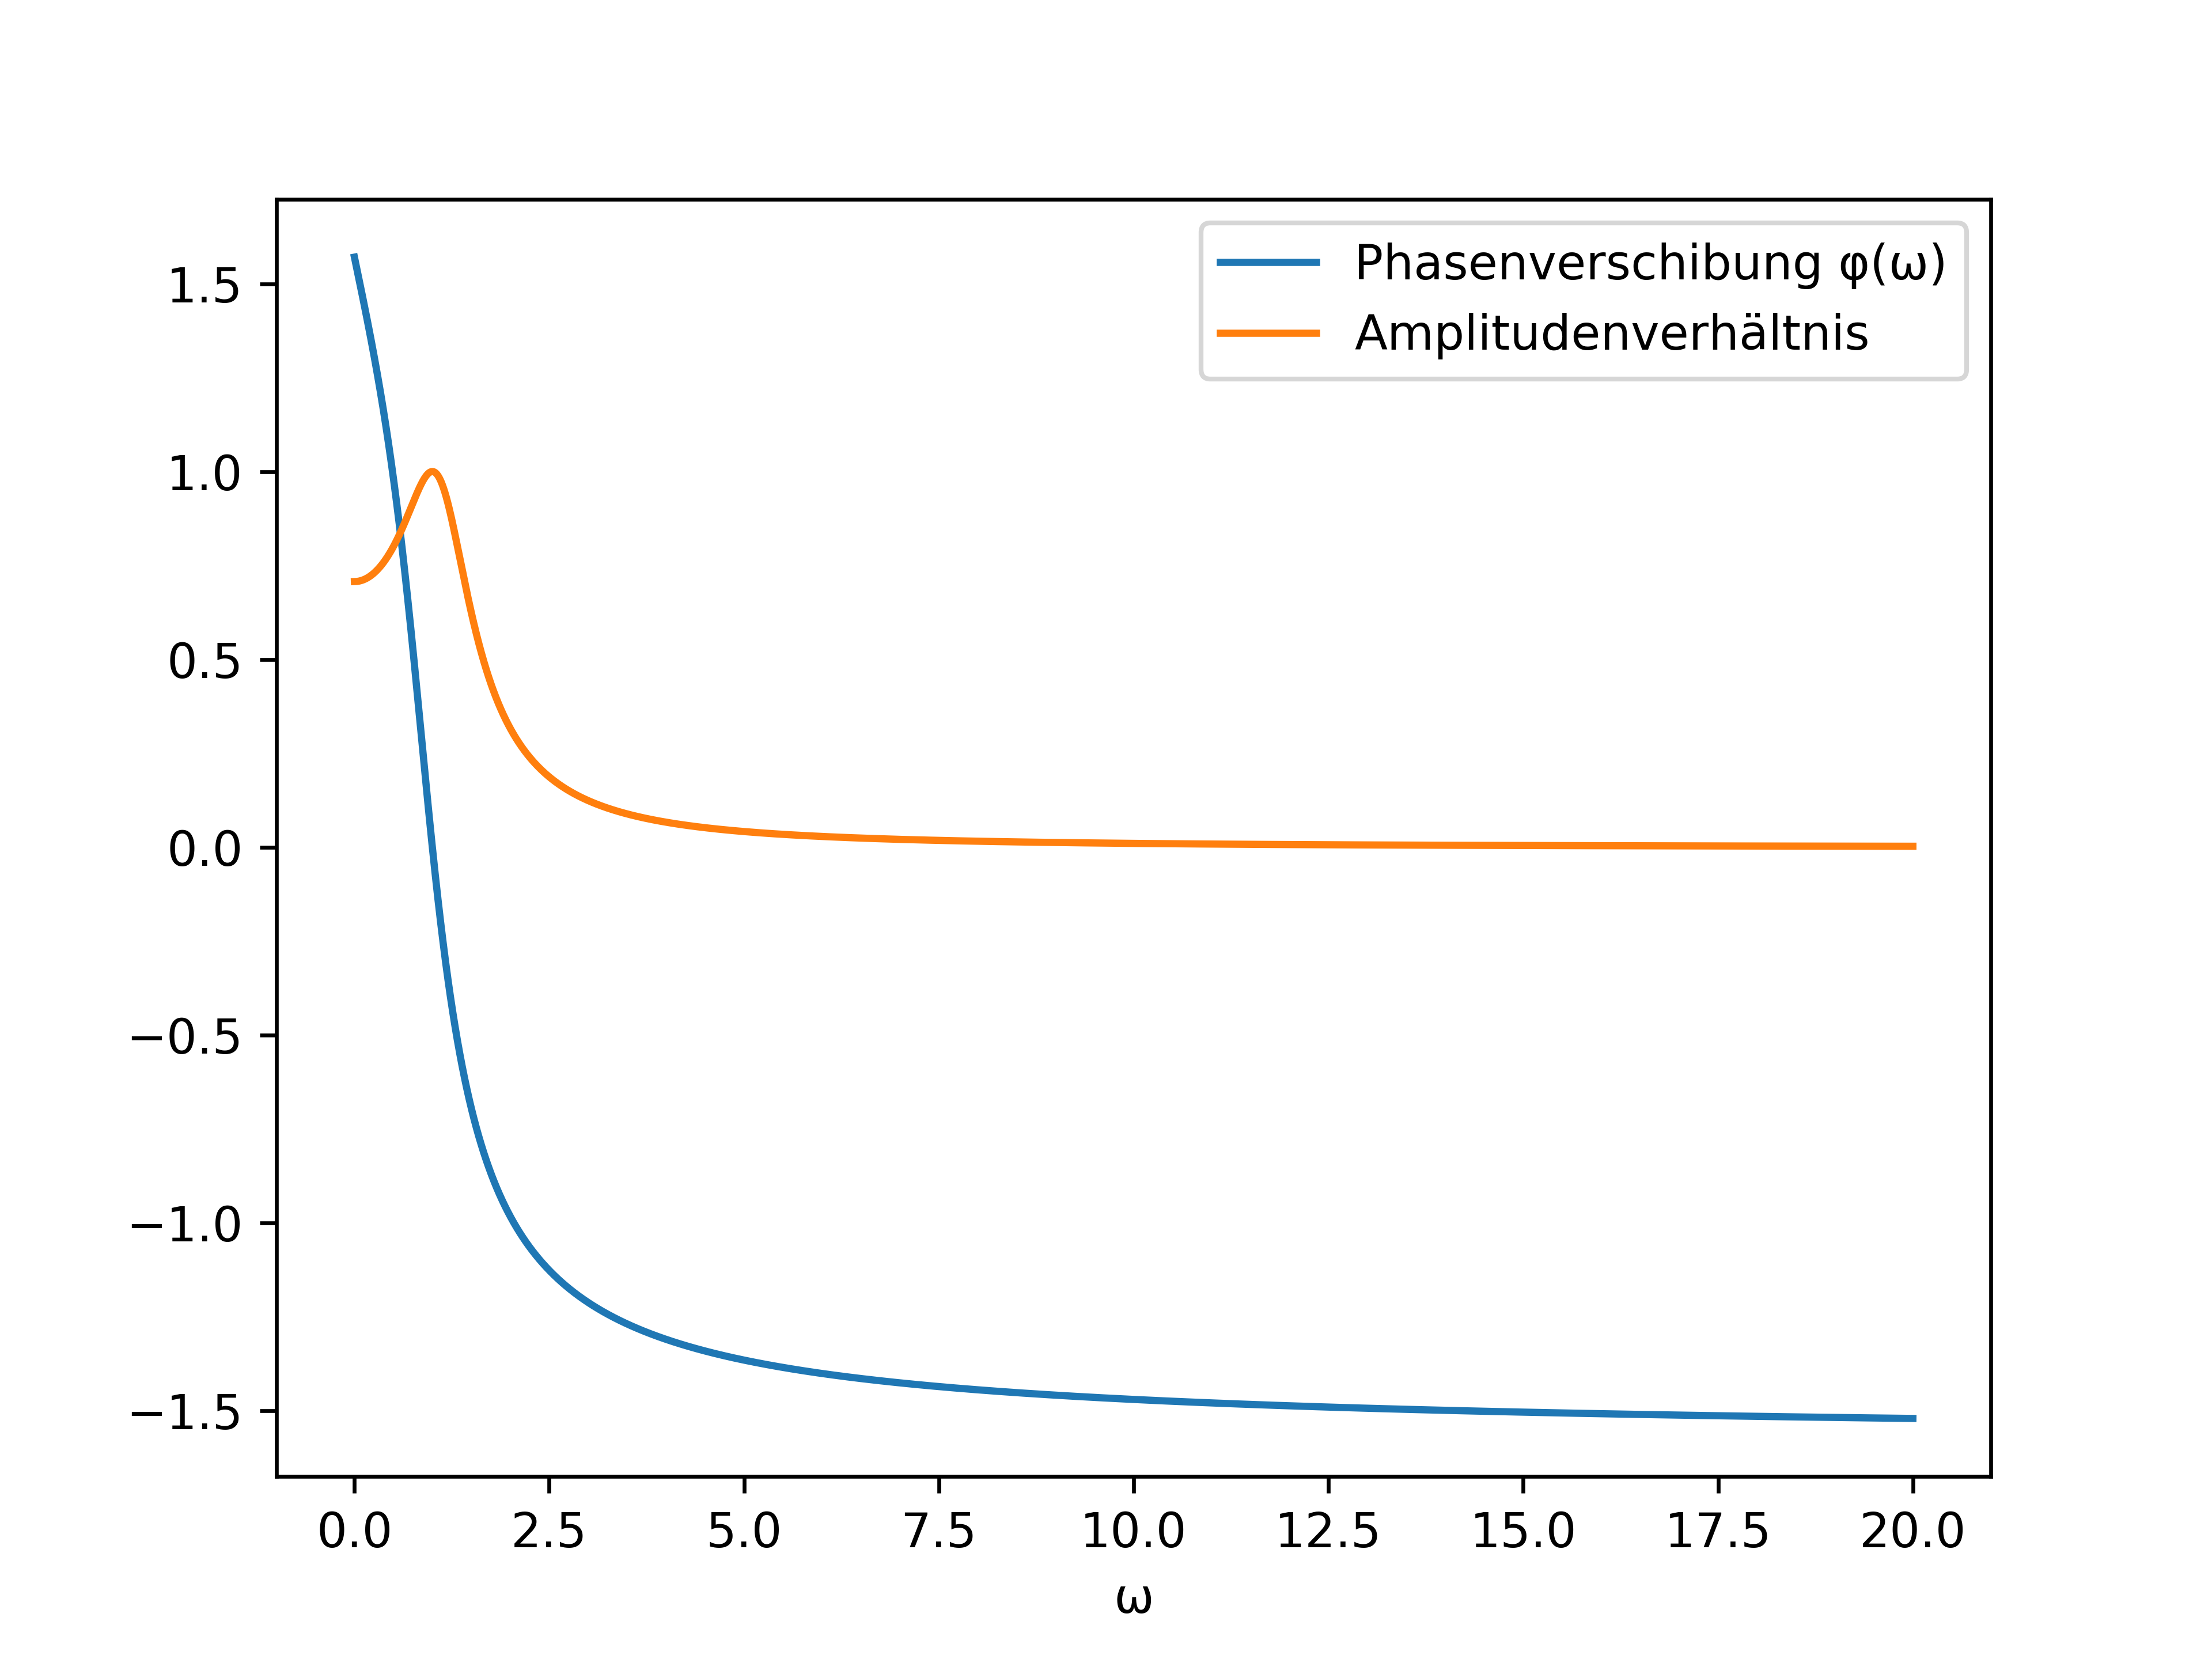
\includegraphics[width=12cm]{aufgabe3.png}
\end{figure}

c) Die für die maximale Spannung gilt:
\[ U_0^\text{max} = \text{max}\vert Z \vert \ I_0 \]
Gesucht wird also ein Maximum von $\vert Z \vert$, bilde dazu die Ableitung und setze diese gleich 0:
\begin{align*}
	\frac{d}{d\omega} \vert Z(\omega) \vert 
	&= \frac{d}{d\omega} \frac{RL}{\sqrt{L^2 + R^2  \left(\frac1\omega - \omega LC \right)^2}} \\
	% linearität ausnutzen
	&= LR \ \frac{d}{d\omega} \left(L^2 + R^2  \left(\frac1\omega - \omega LC \right)^2 \right)^{-0.5} \\
	&= LR \ (-0.5) \left(L^2 + R^2  \left(\frac1\omega - \omega LC \right)^2 \right)^{-1.5}
		\ \frac{d}{d\omega} \left(L^2 + R^2  \left(\frac1\omega - \omega LC \right)^2 \right) \\
	&= LR \ (-0.5) \left(L^2 + R^2  \left(\frac1\omega - \omega LC \right)^2 \right)^{-1.5}
		2R^2  \left(\frac1\omega - \omega LC \right) \cdot \left(-\frac{1}{\omega^2} - LC \right) \\
	% bisschen kuerzen und gleich 0 setzen
	&= LR^3 \ \left(L^2 + R^2  \left(\frac1\omega - \omega LC \right)^2 \right)^{-1.5}
		\left(\frac1\omega - \omega LC \right) \cdot \left(\frac{1}{\omega^2} + LC \right) 
	\overset != 0
\end{align*}
\[
\Leftrightarrow \qquad
	L^2 + R^2  \left(\frac1\omega - \omega LC \right)^2 = 0 \quad \lor \quad
	\frac1\omega - \omega LC = 0 \quad \lor \quad
	\frac{1}{\omega^2} + LC = 0
\]
Die linke und rechte Gleichung besitzen keine Lösung, die mittler liefert durch Umstellen
\[ \omega = \frac 1 {\sqrt{LC}} \]
Der Graph aus b) zeigt uns, dass es sich auch um ein Maximum handelt. \\
Damit benötigt man für die gegebenen Werte maximal
\[ U_0^\text{max} =  \vert Z\left(\sqrt{LC}\right) \vert \ I_0 = R \ I_0 = 10^3 V. \]

\newpage

\section*{Aufgabe 5}

\quad (a) Bei der Schaltung handelt es sich um einen Tiefpass. \\
Bei niedrigen Frequenzen verhält sich die Induktivität 
wie ein normales Kabel ($Z_L \approx 0$), erst bei hohen Frequenzen muss der Strom mehr gegen die 
Selbstinduktivität ``ankämpfen``.
\[ V(\omega) = \frac{R_a}{Z_\text{ges}} = \frac{R_a}{R + R_a + i\omega L} \]
\\

(b) Bei der Schaltung handelt es sich um einen Hochpass. \\
Bei niedrigen Frequenzen nähert sich das Verhalten der
Schaltung der bei Gleichstrom an, wodurch die Impedanz des Kondensators gegen unendlich geht.
\[ V(\omega) = \frac{R_a}{Z_\text{ges}} = \frac{R_a}{R + R_a + \frac{1}{i\omega c}} \]
\\

(c) Die Schaltung ist ein Hochpass. \\
Bei niedrigen Frequenzen würde der meiste Strom nicht durch den Verbraucher, sondern durch die Induktivität laufen.
Erst bei höheren Frequenzen steigt die Impedanz der Induktivität und mehr Strom fließt durch den Verbraucher.
\[
	Z_a = \frac{R_a \ Z_L}{R_a + Z_L} = \frac{R_a \ i\omega L}{R_a + i\omega L} 
	\Rightarrow 
	V(\omega) = \frac{Z_a}{Z_\text{ges}} 
	= \frac{R_a \ i\omega L}{R_a + i\omega L} \frac{1}{R + \frac{R_a \ i\omega L}{R_a + i\omega L}}
	= \frac{\omega L - iR_a}{R R_a \omega L + \omega L - iR_a}
\]
\\

(d) Die Schaltung ist ein Tiefpass. \\
Das Verhalten ist das Umgekehrte zu der bei (c). Hier ist es jedoch so, dass bei niedrigen Frequenzen die Impedanz
des Kondensators gegen unendlich geht und bei hohen Frequenzen durchlässig wird. Dadurch fließt bei tiefen
Frequenzen viel Strom durch den Verbraucher, bei hohen wenig.
\[
	Z_a = \frac{R_a}{1 + R_a i\omega C}
	\Rightarrow 
	V(\omega) = \frac{Z_a}{Z_\text{ges}} 
	= \frac{R_a}{1 + R_a i\omega C} \frac{1}{R + \frac{R_a}{1 + R_a i\omega C}}
	= \frac{R_a}{R + R_a + RR_a i\omega C}
\]
\\

(e) Die Schaltung ist ein Bandpass. \\
Bei hohen Frequenzen ``scheitert`` der Strom an der Induktivität, bei niedrigen an dem Kondensator.
\[
	V(\omega) = \frac{Z_a}{Z_\text{ges}} = \frac{R_a}{R + i\omega L + \frac{1}{i \omega C} + R_a}
\]
\\

(f) Die Schaltung ist ein Sperrfilter. \\
Sehr hohe Frequenzen können einfach durch den Kondensator, niedrige durch die Induktivität. Frequenzen in einem
mittleren Frequenzbereich werden jedoch nicht stark durchgelassen.
\[
	V(\omega) = \frac{Z_a}{Z_\text{ges}} 
	= \frac{R_a}{R + \frac{L}{C} \frac{i\omega C}{1 - \omega^2 LC} + R_a}
\]




\end{document}
